\subsection{CNN - Convolutional Neural Networks}
\label{back:cnn}

\acrfull{cnn} \cite{}, a specialized type of feed-forward neural network, has become a cornerstone in \acrshort{dl} architectures. Building upon simpler structures like the linear layer discussed in section \ref{back:linear}, CNNs introduce a powerful approach to processing matrix data, especially images.
The foundations of CNNs can be traced back to neurobiological research in the 1960s on the visual cortex \cite{hubel1962receptive}, but they were first properly introduced to the \acrshort{ml} field in 1990 by Yan LeCun \cite{NIPS1989_53c3bce6}. Since then, CNNs have undergone significant developments, leading to breakthroughs in various fields of artificial intelligence. \\

\begin{figure}[!h]
    \centering
    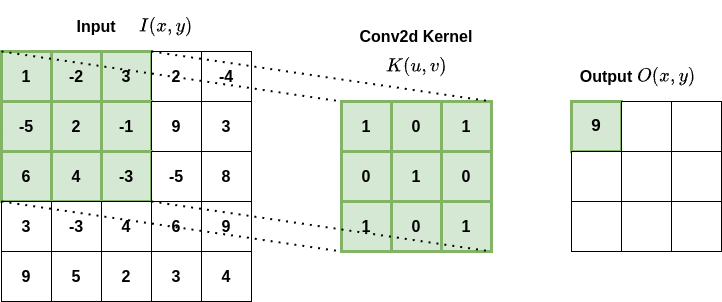
\includegraphics[width=0.8\linewidth]{figures/convolution.png}
    \caption{Example of a 2D Convolutional operation}
    \label{fig:2dconv}
\end{figure}

At their core, CNNs rely on kernel operations, primarily convolutions, to calculate features. The convolution is a mathematically operation which can be defined continuously as following:

\begin{equation}
(f * g)(t) = \int_{-\infty}^{\infty} f(\tau) g(t - \tau) d\tau
\label{eq:contconv}
\end{equation}

and discretely as such:

\begin{equation}
   (f * g)(x, y) = \sum_{m=0}^{M-1} \sum_{n=0}^{N-1} f(m, n)g(x-m, y-n) 
\label{eq:conv}
\end{equation}

Here $f$ is the input matrix, $g$ is the kernel, $m$ and $n$ is the 

The convolutional operation is essentially multiple matrix multiplication between different regions in the data and a kernel. These multiplications can be performed in a parallelized manner. Matrix multiplications have undergone significant improvement over the years CITE, and have with the introduction of CUDA, been further optimized for better suited hardware architectures such as \acrshort{gpu}s. With the rapid improvements of \acrshort{gpu}s, especially by NVIDIA, the computational efficiency of both linear and convolutional layers has improved drastically. This has resulted in overall lower energy requirements for model training, reduced training times and the introduction of distributed large-scale model training \cite{mungoli2023scalable}. \\ 

Unlike fully connected layers that compute global interactions, convolution operations in CNNs focus on local regions data. This localized approach allows for improved feature extraction, making them particularly effective for tasks involving spatial data such as image recognition, object detection, and segmentation. \\


The power of CNNs lies in their ability to automatically learn hierarchical feature representations. Lower layers typically detect simple features like edges or colors, while deeper layers combine these to recognize more complex features. This hierarchical learning, coupled with parameter sharing and local connectivity, enables \acrshort{cnn}s to be both computationally efficient and highly effective at capturing relevant features from high-dimensional data. \\

Due to \acrshort{cnn}s inherent quality of feature extraction, they are not as prone to the vanishing gradient problem \cite{tan2019vanishing} as linear layers. This occurs when gradients propagated backward through the layers become very small, making it difficult for the network to update its weights effectively. \\

Only the size of the kernel is used to stored neurons when performing cross correlation convolution, compared to linear layers where all the weights between layers needs to be stored. \acrshort{cnn}s are highly applicable to numerous different tasks, such as recognition and classification. \\

\subsubsection{Pooling}

Typically, a convolution is followed by an activation function $f$ and then a pooling operation. A pooling operation works like a filter $k$, selecting a certain value from a subset of the input vector based on a heuaristic. The three most common operations are \textit{max pool}, \textit{min pool} and \textit{avg pool}. Out of these, the \textit{max pool} operation operation is most commonly used. This operation reduces dimensionality, outputting only the most important feature for future layers. \\

\begin{figure}[!h]
    \centering
    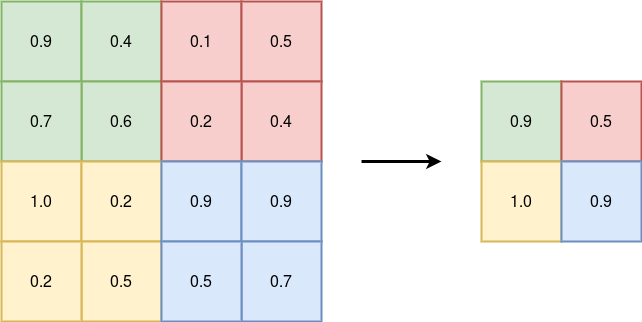
\includegraphics[scale=0.4]{figures/pooling.png}
    \caption{Example of a $2 x 2$ max pool operation with stride 2}
    \label{fig:maxpool}
\end{figure}

In figure \ref{fig:maxpool}, we see an input matrix $M$ where each 2x2 submatrix is being filtered by choosing the maximum element $\hat{M}_{max}$. The filter then strides across $M$ by two elements, repeating the operation until $M$ has been completely filtered.